\section{Experiments and Evaluation}
We conduct several experiments for all four settings to evaluate the influence of order awareness and availability of dependency type information to the similarity prediction performance. In the following, we describe the dataset and the hyperparameter setting. Finally, we present the results and an analysis of errors.

\subsection{Dataset}
We use the SICK corpus\footnote{\url{http://alt.qcri.org/semeval2014/task1/index.php?id=data-and-tools}} \autocite{marelli_sick_2014} for model training and evaluation. The corpus consists of about approximately 10.000 pairs of English sentences based on the 8K ImageFlickr data set\footnote{\url{http://nlp.cs.illinois.edu/
HockenmaierGroup/data.html}} \autocite{hodosh_framing_2013} and the SemEval 2012 STS MSR-Video Description data set\footnote{\url{https://www.cs.york.ac.uk/semeval-2012/task6/index.php\%3Fid=data.html}} \autocite{agirre_semeval-2012_2012} that contain sentences describing the same picture or video. These sentences were linguistically normalized, so Named Entities and complex verb constructions are replaced or subordinates are turned into coordinates, for instance. Furthermore, they are manually expanded to generate candidate pairs that were labeled by 5 annotators with one to five point relatedness ratings that are averaged to produce a relatedness score. We rescaled the scores into the interval $[0.0, 1.0]$ to let them fit into our definition of a similarity measure. Table~\ref{tab:sick_examples} shows some examples of the dataset. The mean of the score for both train and test set is approximately $0.63$. The sentences have an average length of $9.6$ words and contain $2408$ different token types.  
%mean score: 0.63 * 4.0 + 1.0 = 3.53
\todo{AB:explain why SICK}

\begin{table*}[!htb]
\centering
  \begin{tabular}{p{0.4\textwidth}|p{0.4\textwidth}|c}
    sentence A & sentence B & score \\ \hline \hline
    A man in a shirt dyed purple is looking at a man in a black shirt who is doing a funny face & A man in a shirt dyed purple is looking at a man in a black shirt who is doing a face which looks funny & 1.0 \\ \hline
    A group of kids is playing in a yard and an old man is standing in the background & A group of boys in a yard is playing and a man is standing in the background & 0.875 \\ \hline
    A brown dog is attacking another animal in front of the man in pants & Two dogs are wrestling and hugging & 0.55 \\ \hline
    A woman is chopping an onion & A woman is washing her feet & 0.0
  \end{tabular}
  \caption{Example sentence pairs from SICK corpus with rescaled relatedness score ranging from $0.0$ (not related) to $1.0$ (maximal related).}
\label{tab:sick_examples}
\end{table*}

%\subsubsection{SICK}

%\subsubsection{PPDB}
%Our pre-training dataset is based on the phrasal part of the PPDB 2.0 dataset \autocite{pavlick_ppdb_2015}. We use a subset of 100,000 paraphrases and add an equal amount of negative samples by replacing for each pair the second paraphrase entry with a random phrase sampled uniformly\footnote{We also tried to sample according to the Jaccard similarity distribution of the original pairs, but this decreased the performance.} from all existing second pair entries. A similarity score of 1.0 is assigned to the original paraphrase pairs, the negative samples are scored with 0.0.

\subsection{Training and Hyperparameters}
We train the model in batches of 100 examples. The ADAM optimizer is initialized with a learning rate of 0.003. We apply gradient clipping by global norm as specified in \textcite{pascanu_difficulty_2012} with a threshold of 5.0 and use dropout \autocite{srivastava_dropout_2014} with a keep probability of 0.8 at the \ac{LSTM} and the \ac{FC} in the \ac{AVG} case to prevent from overfitting. We used a grid search at the train/dev set to find this parameter configuration. We applied 5-fold cross validation with regard to the train/dev split for every setting and repeated each experiment 10 times to achieve robust results.

\subsection{Results}
We measured performance using the Pearson correlation coefficient and \ac{MSE} between the predictions and gold scores. The mean Pearson correlation of all runs is about $0.839$ with a \ac{std} of $0.002$ and the mean \ac{MSE} is $0.024$ with std of $0.004$. The \ac{TF-IDF} baseline produces a Pearson score of $0.619$ and a \ac{MSE} of $0.082$. All scores averaged over same parameter settings are shown in Table~\ref{tab:results}. Figure~\ref{subfig:res_sep_mse} displays the \ac{MSE} and Pearson's r results for all parameter combinations as box plots\footnote{The boxes of all box plots show the \ac{IQR}, whiskers mark the $[1.5\times \text{IQR}, 3\times \text{IQR}]$ range and notches the  $10000\times$ bootstrapped confidence intervals.}. Note, that the y-axis is inverted for all box plots visualizing \ac{MSE} scores to show better performing scores above worse ones and to provide comparability with plots of Pearson scores. 
%# SICK_VERBADJNOUN_lemma	0.611	0.091		# TFIDF
%# SICK_ADJNOUN_lemma	0.558	0.111			# TFIDF
%# SICK_VERBADJNOUN_orth	0.568	0.106		# TFIDF
%# SICK_ADJNOUN_orth	0.542	0.119			# TFIDF

%\begin{figure}[htb!]
%  \centering
%  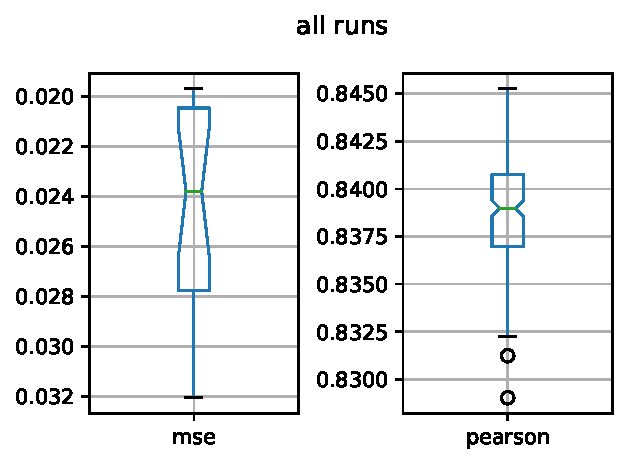
\includegraphics[width=0.9\textwidth]{results/fig_merged.pdf}
%  \caption{Overall model performance as Pearson correlation and MSE.}
%  \label{fig:res_merged}
%\end{figure}

%\begin{figure}[htb!]
%  \centering
%  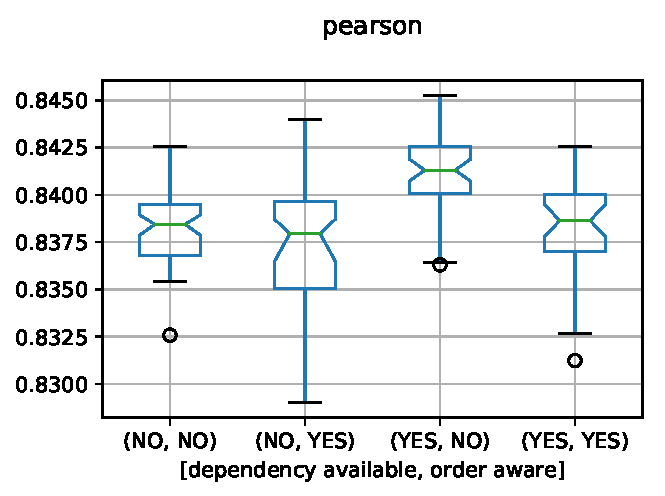
\includegraphics[width=0.9\textwidth]{results/fig_sep_pearson.pdf}
%  \caption{Pearson correlation scores for the different settings.}
%  \label{fig:res_sep_pearson}
%\end{figure}

%\begin{subtable}[c]{\textwidth}
%	\centering
\begin{table}[htb!]
  	\centering
  	%\begin{tabular}{|l|l|l|}
 \begin{tabularx}{\textwidth}{|X X|X|X|}
 %\begin{tabularx}{\textwidth}{|p{0.21\textwidth} p{0.15\textwidth}|X|X|} %{p{0.4\textwidth}|p{0.4\textwidth}|c}
		\hline
		dependency type & order aware & mse & pearson \\ \hline \hline
		NO & NO & 0.0284 & 0.8382 \\ 
		NO & YES & 0.0206 & 0.8375 \\
		YES & NO & 0.0274 & 0.8413 \\
		YES & YES & 0.0205 & 0.8383 \\ \hline \hline
		\multicolumn{2}{|l|}{TFIDF} & 0.0823 & 0.6189 \\ \hline
 \end{tabularx}
 %\captionsetup{width=0.9\linewidth}
 \caption{MSE and Pearson scores aggregated by setting.}
 \label{tab:results}
\end{table}
%	\vspace*{0.8 cm} \newline
	
  %\caption{Average \ac{MSE} and Pearson's r scores}
%\end{table}


\begin{figure}[htb!]
  \centering
  \textbf{Overall performance by setting}\par\medskip
  \begin{subfigure}{.5\textwidth}
    \centering
    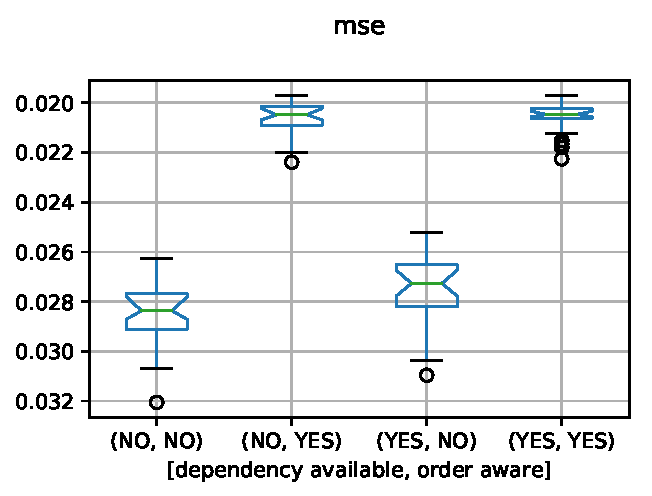
\includegraphics[width=1.\linewidth]{results/fig_sep_mse.pdf}
    \captionsetup{width=0.9\linewidth}
    \caption{MSE for the different settings (inverted y-axis).}
    \label{subfig:res_merged}
  \end{subfigure}%
  \begin{subfigure}{.5\textwidth}
    \centering
    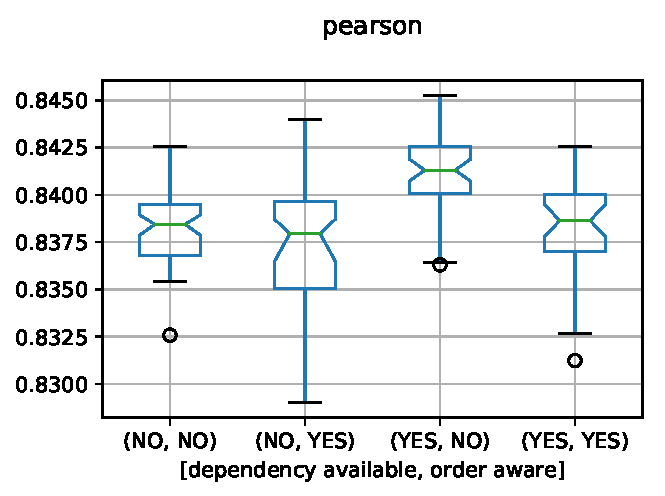
\includegraphics[width=1.\linewidth]{results/fig_sep_pearson.pdf}
    \captionsetup{width=0.9\linewidth}
    \caption{Pearson's r for the different settings.}
    \label{subfig:res_sep_mse}
  \end{subfigure}
  %\caption{A figure with two subfigures}
  \label{fig:res_all}
\end{figure}

Enabling the feature \textbf{order aware} results in a significant overall performance gain of $0.75\%$ in means of \ac{MSE} and a performance decrease of $-0.21\%$ with regard to Pearson's r ($p<0.0001$ for two-tailed t-test \todo{AB:ref?} in both cases). Adding \textbf{dependency types} improves the overall \ac{MSE} by $0.05\%$ and Pearson's r increases by $0.24\%$, whereby the former is not significant (p=0.336), but the later is ($p<0.0001$). Table~\ref{tab:results_merged} shows the specific scores.


\begin{table}[htb!]
	\centering
	\begin{tabularx}{\textwidth}{|p{0.25\textwidth} p{0.15\textwidth}|X X|X X|} 
		%\begin{tabularx}{\textwidth}{|p{0.21\textwidth} X|X|X|} %{p{0.4\textwidth}|p{0.4\textwidth}|c}
		\hline
		parameter & enabled & mse & & pearson  & \\ \hline \hline
		dependency type & NO & 0.0245 & & 0.8378 & \\
		dependency type & YES & 0.0240 & $+0.05\%$* & 0.8398 & $+0.24$\% \\ \hline
		order aware & NO & 0.0279 &  & 0.8397 &  \\
		order aware & YES & 0.0206 & $+0.75\%$ & 0.8379 & $-0.21\%$ \\ \hline	   		
	\end{tabularx}
	%\captionsetup{width=0.9\linewidth}
	\caption{Scores aggregated by individual parameter assignment and percentage improvement when enabling the feature. The improvement marked with (*) is not significant.}
	\label{tab:results_merged}
\end{table}

\subsubsection{Relation of Order awareness and Dependency types}

\begin{figure}[htb!]
  \centering
  \textbf{Order awareness}\par\medskip
  \begin{subfigure}{.5\textwidth}
    \centering
    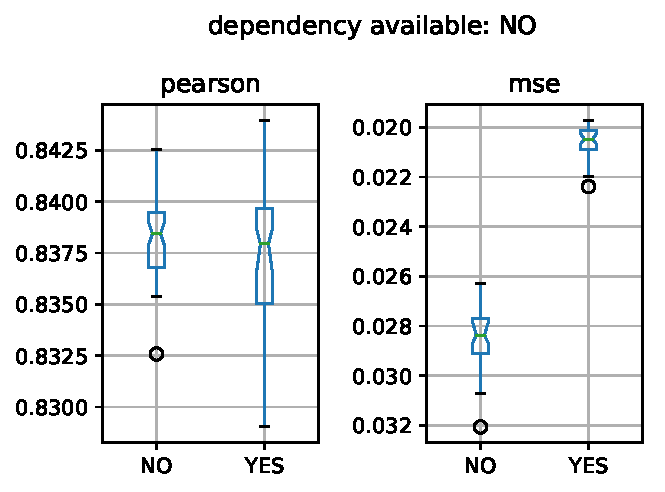
\includegraphics[width=1.\linewidth]{results/fig_sep_cond_dependencyNO.pdf}
    %\captionsetup{width=0.9\linewidth}
    %\caption{Impact of parameter \textit{order aware} conditioned by disabled \textit{dependency available} parameter.}
  \end{subfigure}%
  \begin{subfigure}{.5\textwidth}
    \centering
    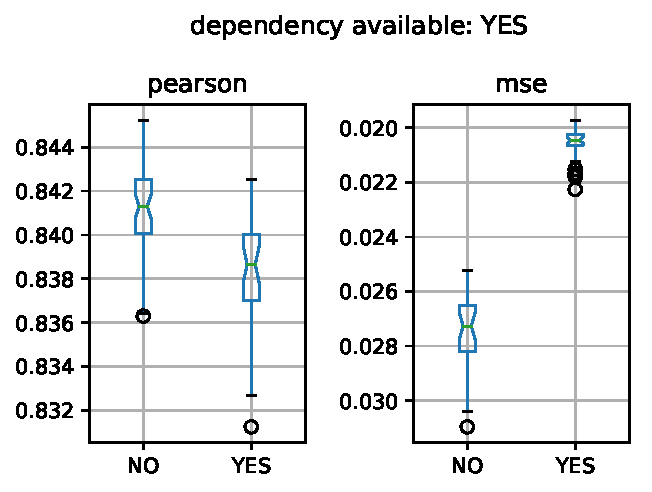
\includegraphics[width=1.\linewidth]{results/fig_sep_cond_dependencyYES.pdf}
    %\captionsetup{width=0.9\linewidth}
    %\caption{Impact of parameter \textit{order aware} conditioned by enabled \textit{dependency available} parameter.}
  \end{subfigure}
  \caption{Impact of parameter \textit{order aware} conditioned by parameter \textit{dependency available}.}
  \label{fig:fig_sep_order}
\end{figure}


%\begin{figure}[htb!]
%  \centering
%  \includegraphics[width=0.9\textwidth]{fig_sep_order.pdf}
%  \caption{Influence of order awareness measured with Pearson correlation and MSE.}
%  \label{fig:pearson_all_sep}
%\end{figure}

%\subsubsection{cosine vs. manhattan}
%\subsubsection{Dependency edge types}
%mean mse: 0.0245 -> 0.0240 =  -0.0005 \\
%mean pearson: 0.8378 -> 0.8398 =   0.0019 \\
%performance gain of 0,05\%*/0,31\% (mse/pearson) regarding TF-IDF baseline 

%*: not significant
%\begin{figure}[htb!]
%  \centering
%  \includegraphics[width=0.9\textwidth]{fig_sep_dep.pdf}
%  \caption{Influence of dependency edge type Information measured with Pearson correlation and MSE.}
%  \label{fig:pearson_all_sep}
%\end{figure}

\begin{figure}[htb!]
\centering
\textbf{Dependency types}\par\medskip
\begin{subfigure}{.5\textwidth}
  \centering
  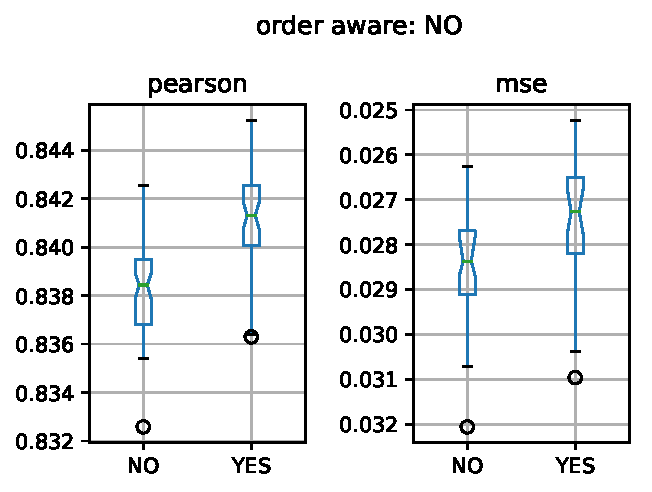
\includegraphics[width=1.\linewidth]{results/fig_sep_cond_orderNO.pdf}
  %\captionsetup{width=0.9\linewidth}
  %\caption{Impact of parameter \textit{dependency available} conditioned by disabled \textit{order aware} parameter.}
  %\label{fig:sub1}
\end{subfigure}%
\begin{subfigure}{.5\textwidth}
  \centering
  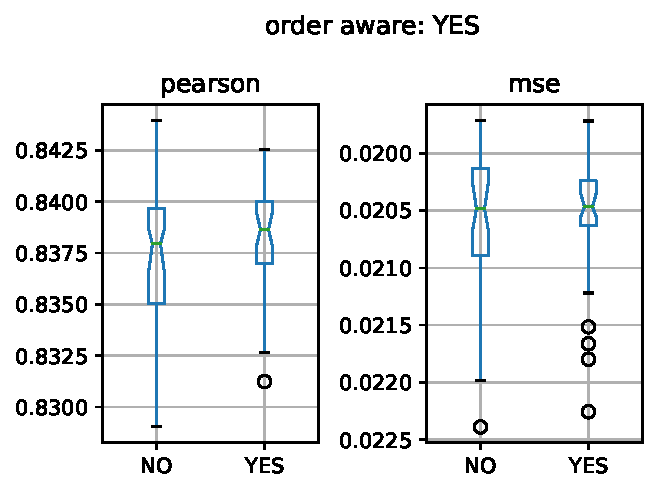
\includegraphics[width=1.\linewidth]{results/fig_sep_cond_orderYES.pdf}
  %\captionsetup{width=0.9\linewidth}
  %\caption{Impact of parameter \textit{dependency available} conditioned by enabled \textit{order aware} parameter.}
  %\label{fig:sub2}
\end{subfigure}
\caption{Impact of parameter \textit{dependency available} conditioned by parameter \textit{order aware}.}
\label{fig:fig_sep_dep}
\end{figure}

%\subsubsection{Pretraining}

\subsubsection{Qualitative error analysis}

\begin{figure}[htb!]
  \centering
  \textbf{deviations from gold scores}\par\medskip
  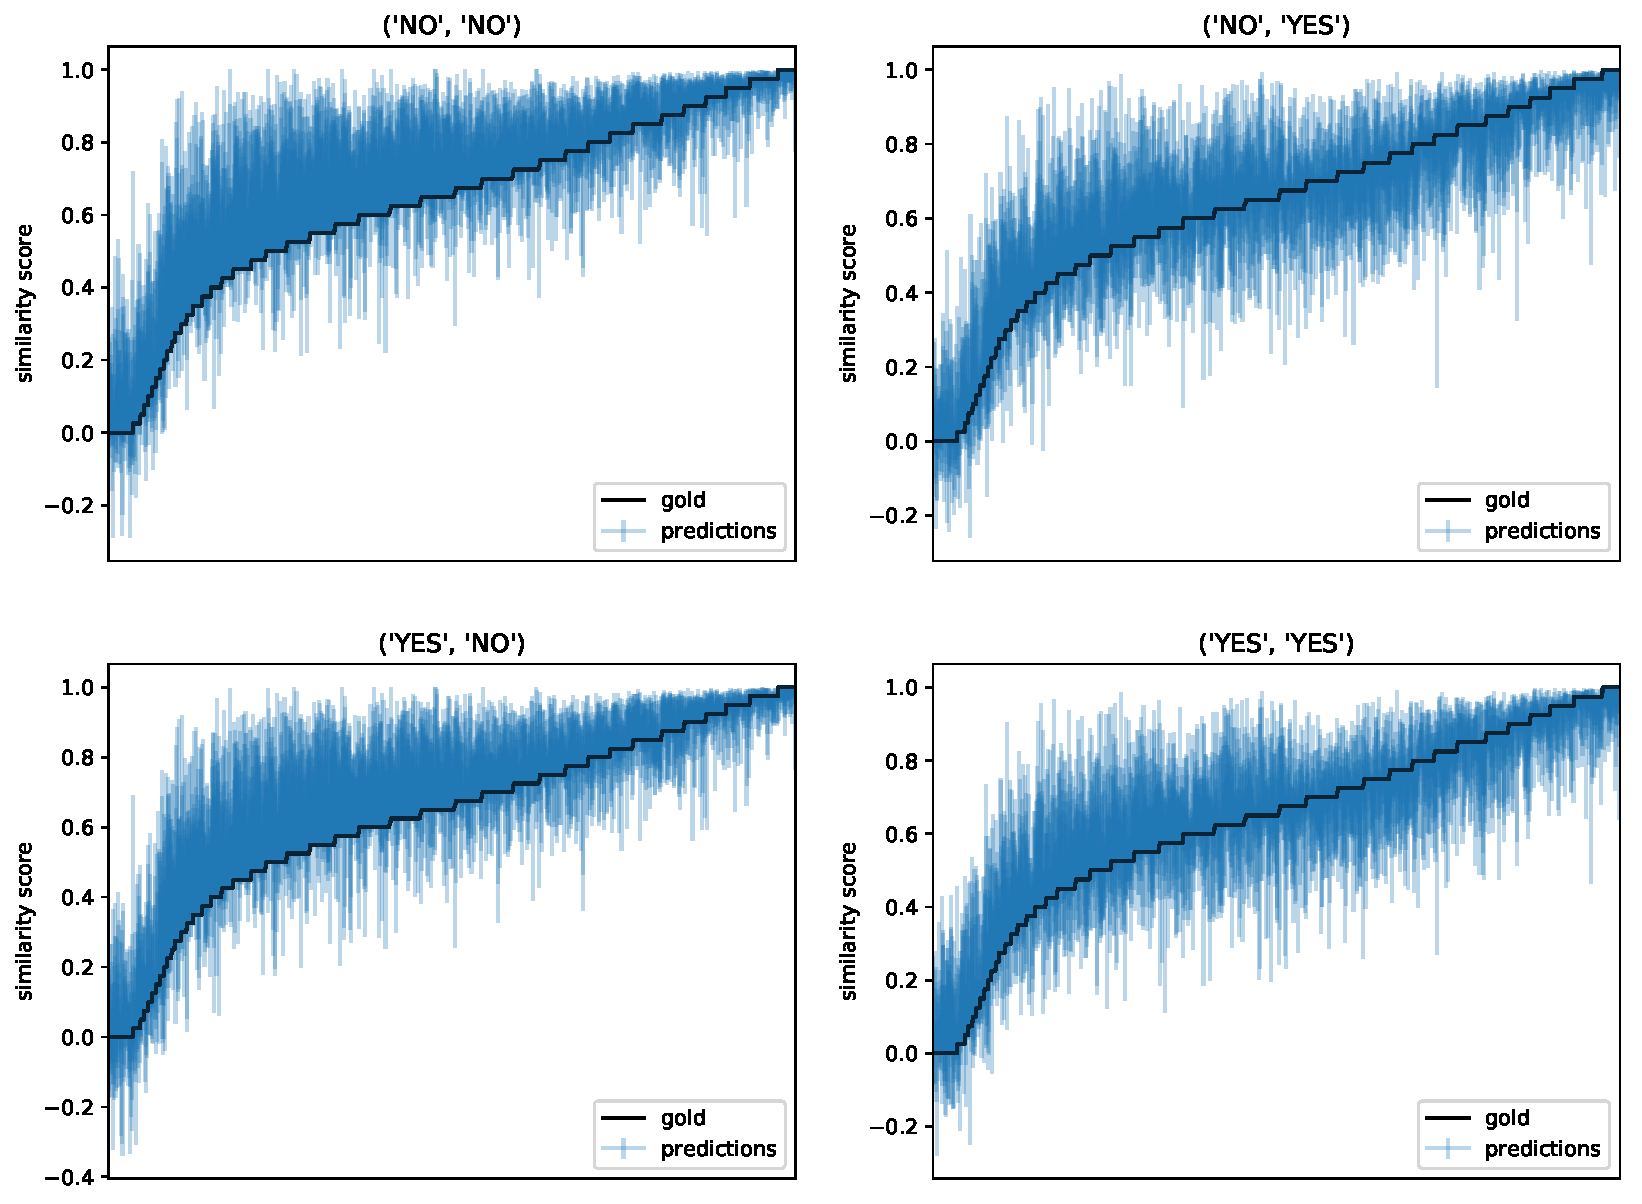
\includegraphics[width=1.\linewidth]{results/fig_sorted_errors_sep.pdf}
  \caption{Deviations of the predictions from gold similarity scores by setting (<dependency available>, <order aware>)}
  \label{fig:fig_sorted_errors_sep}
 \end{figure}

% Alternations / Diathese
%http://ling.uni-konstanz.de/pages/home/hautli/LR/verb-classes-levin.pdf
%http://ccl.pku.edu.cn/973_sem_spec/Sem_ling/English%20Verb%20Classes%20and%20Alternations%20A%20Preliminary%20Investigation.pdf

% pearson-correlation("('NO', 'NO') vs ('YES', 'NO') abs"; "score_jaccard") = -0.456
% > increasing overlap -> decreasing benefit of "dependency available" 
